% \setcounter{secnumdepth}{2}

\chapter{Hito 1: Definición del problema y determinación del alcance}

En este capítulo se detalla la definición del problema seleccionado para la evaluación del proyecto de la asignatura \textit{Desarrollo e Integración de Servicios de IA}, así como la determinación de su alcance.

\section{Contexto y definición del problema}

En el ámbito de las plataformas digitales de relaciones interpersonales, la predicción de compatibilidad entre individuos constituye un problema de \textbf{alta relevancia tecnológica, social y económica}. Las aplicaciones de citas modernas gestionan grandes volúmenes de información estructurada sobre los usuarios, incluyendo variables demográficas, profesionales, rasgos de personalidad y preferencias relacionales. A partir de estos datos, los sistemas deben decidir qué perfiles recomendar y qué emparejamientos priorizar.\\

La compatibilidad relacional es, sin embargo, un \textbf{fenómeno inherentemente complejo y multidimensional}. No depende exclusivamente de variables superficiales como la edad o la localización geográfica, sino que está influida por la interacción entre rasgos de personalidad, valores personales, ambiciones profesionales, estilos de comunicación, hábitos cotidianos y expectativas afectivas. Esta naturaleza multifactorial convierte la modelización de la compatibilidad en un problema analítico no trivial.\\

Tradicionalmente, muchas plataformas han empleado reglas heurísticas o sistemas de filtrado simples basados en coincidencias directas. Estos enfoques presentan limitaciones evidentes, especialmente en escenarios donde las interacciones entre variables son no lineales y complejas: no capturan interacciones complejas, no aprenden patrones implícitos y carecen de transparencia. A diferencia de una regla heurística simple que podría asumir erróneamente que dos personas con la misma \textit{ambición profesional} son compatibles, un modelo de inteligencia artificial puede descubrir \textbf{patrones latentes}. Por ejemplo, identificar que dos personas con niveles opuestos de \textit{espontaneidad} pueden ser altamente compatibles si comparten el mismo \textit{lenguaje del amor}. Esta capacidad de capturar interacciones no lineales justifica la necesidad de emplear algoritmos avanzados.\\

El dataset seleccionado para este proyecto, \textit{“Cupid’s Algorithm”}~\cite{dataset_cupid}, contiene información estructurada sobre pares de individuos (Person A – Person B), incluyendo:

\begin{itemize}
    \item \textbf{Variables demográficas} (edad, nivel educativo, localización).
    \item \textbf{Variables profesionales} (campo profesional, nivel de ambición).
    \item \textbf{Rasgos de personalidad} basados en el modelo \textit{Big Five}.
    \item \textbf{Variables relacionales} (lenguaje del amor, cronotipo, espontaneidad, expresividad emocional).
    \item Una variable continua de compatibilidad ($compatibility\_score$).
    \item Una variable binaria de compatibilidad ($compatible$).
    \item Un indicador de longevidad relacional ($relationship\_longe$).
\end{itemize}

La presencia de estas variables permite abordar el problema desde una \textbf{perspectiva supervisada}, donde la compatibilidad observada actúa como señal objetivo para el aprendizaje.

Desde el punto de vista formal, el problema puede plantearse como un problema de 
\textbf{clasificación binaria}~\cite{geron2019hands}. Cada par de individuos queda 
caracterizado por un conjunto de variables numéricas y categóricas que describen 
sus atributos individuales.

Sea $X \in \mathbb{R}^n$ el vector de características construido a partir de las 
variables de ambos individuos. El sistema debe aprender una función parametrizada:

\[
f_\theta : \mathbb{R}^n \rightarrow [0,1]
\]

tal que:

\[
\hat{y} = f_\theta(X) = P(Y=1 \mid X)
\]

donde $Y=1$ indica compatibilidad entre los individuos.

De este modo, el modelo estima la probabilidad de que un determinado par 
de individuos sea compatible, en función de las interacciones existentes 
entre sus características demográficas, profesionales y psicológicas.

Alternativamente, el problema puede formularse como una regresión (utilizando $compatibility\_score$) o como una predicción de duración (empleando $relationship\_longe$). No obstante, en este proyecto se delimita el alcance principal al problema de clasificación binaria, al tratarse de una formulación clara, evaluable y directamente alineada con aplicaciones reales de \textit{matching}.\\

El sistema no debe limitarse a generar una predicción numérica, sino que debe concebirse como un \textbf{sistema de inteligencia artificial integrable} en un entorno software real. Esto implica que el modelo debe ser reproducible, evaluable mediante métricas adecuadas y \textit{explicable}, dado que en sistemas que influyen en decisiones sociales la interpretabilidad resulta fundamental para evitar modelos opacos o de tipo ``caja negra''

En consecuencia, el problema queda claramente delimitado: a partir de datos estructurados que describen características personales, profesionales y psicológicas de dos individuos, se busca diseñar un sistema de inteligencia artificial capaz de predecir de forma \textbf{objetiva, consistente y explicable} su compatibilidad relacional, concebido como un componente integrable dentro de una arquitectura software más amplia.

\section{Objetivos generales y específicos}

El problema que se aborda en este proyecto puede formularse de la siguiente manera: ¿Cómo diseñar un sistema de inteligencia artificial capaz de predecir de forma objetiva, consistente y explicable la compatibilidad entre dos individuos, a partir de variables demográficas, profesionales y de personalidad, garantizando su integración como servicio software en una plataforma digital de relaciones?\\

Esta formulación no se limita a la obtención de buenas métricas técnicas, sino que incorpora explícitamente la dimensión de \textbf{sistema IA como producto}, concebido para integrarse en un entorno real, evolucionar en el tiempo y aportar valor a distintos \textit{stakeholders}.\\

Para dar respuesta a esta pregunta, se establece como \textbf{objetivo general} del proyecto diseñar, implementar y validar un sistema de inteligencia artificial capaz de predecir la compatibilidad relacional entre dos individuos utilizando datos estructurados, garantizando su integración en una arquitectura software real y su funcionamiento fiable, explicable y reproducible a lo largo del tiempo.\\

Para alcanzar el objetivo general propuesto, se establecen los siguientes \textbf{objetivos específicos}:

\begin{itemize}
    \item \textbf{Analizar y formalizar} el concepto de compatibilidad relacional desde una perspectiva cuantitativa y multidimensional, identificando las variables más relevantes.
    \item \textbf{Seleccionar y procesar} los datos del dataset \textit{Cupid’s Algorithm}, incluyendo limpieza, codificación y construcción de variables derivadas (similitud o distancia entre perfiles).
    \item \textbf{Diseñar y entrenar} modelos de aprendizaje automático supervisado que permitan predecir la variable binaria compatible, evaluando distintas aproximaciones metodológicas.
    \item \textbf{Evaluar el rendimiento} de los modelos mediante métricas técnicas adecuadas para clasificación binaria (Accuracy, Precision, Recall, F1-score, ROC-AUC), analizando su comportamiento desde una perspectiva de dominio.
    \item \textbf{Incorporar mecanismos de explicabilidad}, que permitan interpretar la influencia relativa de las distintas variables y facilitar su comprensión por parte de perfiles no técnicos.
    \item \textbf{Diseñar el sistema como un servicio integrable}, desarrollando una API REST que permita realizar predicciones de compatibilidad a partir de nuevos pares de individuos.
    \item \textbf{Analizar la viabilidad} económica y organizativa del sistema, estimando costes de desarrollo y potencial retorno de la inversión (ROI).
    \item \textbf{Diseñar el sistema con una arquitectura extensible} que permita, en iteraciones futuras, transicionar de una clasificación binaria a un motor de recomendación Top-K o a la predicción de longevidad relacional.
\end{itemize}

De este modo, el proyecto no se concibe como un simple ejercicio de modelado predictivo, sino como el desarrollo completo de un \textbf{sistema de inteligencia artificial entendido como producto tecnológico}, recorriendo todas las fases de su ciclo de vida.

La Figura \ref{fig:objetivos_coremp} resume el flujo metodológico seguido en el
desarrollo del sistema CORE-MP.

\begin{figure}[h]
\centering
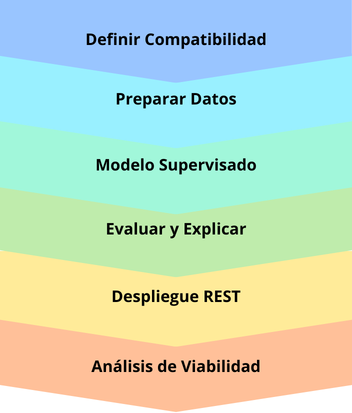
\includegraphics[width=0.7\textwidth]{Pictures/Objetivos.png}
\caption{Flujo metodológico del sistema CORE-MP desde la definición del problema hasta el análisis de viabilidad.}
\label{fig:objetivos_coremp}
\end{figure}


\section{Determinación del alcance}

En esta sección se define el alcance del proyecto a desarrollar en la asignatura, prestando especial atención a los componentes clave que delimitan un sistema de inteligencia artificial concebido como producto: \textbf{planificación temporal, organización del equipo, viabilidad económica y valor generado}.\\

El alcance no solo determina qué se va a desarrollar, sino también qué queda explícitamente fuera del proyecto, con el fin de garantizar su viabilidad dentro del marco temporal y evitar una expansión descontrolada de requisitos.

\subsection{Planificación}

El desarrollo del proyecto se ha estructurado en un horizonte temporal estimado de \textbf{ocho semanas}, concebido como un flujo de trabajo continuo que abarca todas las fases del ciclo de vida de un sistema de \textit{Machine Learning}. Durante las dos primeras semanas, el equipo se centrará en el \textbf{análisis y comprensión del problema}. Esta fase inicial es crítica e implica un estudio detallado del dataset \textit{Cupid’s Algorithm}, la realización de un análisis exploratorio de las variables disponibles y la formalización definitiva del reto como un problema de clasificación binaria.\\

A continuación, las semanas tercera y cuarta se destinarán a la \textbf{preparación y transformación de los datos}. En este periodo se llevarán a cabo tareas fundamentales como la limpieza del conjunto de datos, el tratamiento de valores nulos, la codificación de las variables categóricas y, de forma muy destacada, la ingeniería de características para construir variables derivadas que representen similitudes, diferencias y distancias entre los perfiles. Esta fase concluirá con la división técnica del dataset en conjuntos de entrenamiento y validación.\\

Posteriormente, el proyecto entrará en su núcleo analítico durante las semanas quinta y sexta, enfocadas en el \textbf{modelado y la evaluación}. Durante esta etapa, se entrenarán distintos modelos de aprendizaje supervisado, se compararán sus métricas de rendimiento y se seleccionará el modelo final. Además, se dedicará un esfuerzo específico al análisis de la explicabilidad del sistema, garantizando que las predicciones no provengan de una caja negra. Una vez consolidado el modelo, la séptima semana marcará la transición hacia la \textbf{integración como servicio}. El equipo procederá a la serialización del modelo entrenado y al desarrollo de una API REST que permita realizar predicciones en tiempo real, finalizando con pruebas funcionales del sistema.\\

Finalmente, la octava semana estará dedicada a la \textbf{validación y el análisis de valor}. En esta última etapa se evaluará el sistema en su conjunto, se realizará el análisis de viabilidad económica y retorno de inversión (ROI), y se consolidará la redacción de la documentación final del proyecto, asegurando que el producto técnico cumpla con los estándares académicos y profesionales exigidos.

\subsection{Recursos Humanos: asignación de tareas y capacidad}

El desarrollo del sistema \textbf{CORE-MP} se lleva a cabo mediante la colaboración de un equipo técnico formado por cuatro integrantes. Para garantizar el éxito del proyecto y simular un entorno profesional realista, se han definido perfiles con responsabilidades claramente delimitadas, alineadas con los roles habituales en el desarrollo de productos basados en inteligencia artificial.\\

\textbf{Óscar Domínguez Ocaña. Rol principal: Product Manager y Analista de Negocio.} Dado que el equipo no cuenta de forma nativa con un experto de dominio puro en psicología relacional, este integrante asume un rol híbrido fundamental. Su responsabilidad es actuar como puente entre el desarrollo técnico y los objetivos funcionales del proyecto. Se encarga de comprender a fondo la naturaleza de los datos disponibles, definir qué variables tienen sentido lógico agrupar o comparar, y establecer los umbrales de éxito del sistema. Además, evalúa si los resultados del modelo y su explicabilidad son coherentes y aportan valor real para una hipotética plataforma de \textit{matching}, validando el producto desde la perspectiva del usuario final.\\

\textbf{José Alberto Seco Sánchez-Camacho. Rol principal: Analista de Datos (Data Analyst / Data Engineer).} Este integrante asume la responsabilidad crítica del procesamiento, limpieza y transformación de los datos procedentes del dataset original. Su trabajo abarca desde la exploración estadística inicial hasta la generación de un conjunto de datos consistente y estructurado, aplicando técnicas de ingeniería de características para crear métricas de similitud entre los perfiles. Este rol es la base sobre la que se asienta todo el proyecto, ya que la calidad de las predicciones dependerá directamente de la robustez de los datos preparados en esta fase.\\

\textbf{José Manuel Bastante Rodríguez. Rol principal: Ingeniero de Machine Learning (ML Engineer).} Este perfil es el responsable del diseño metodológico del sistema desde el punto de vista del modelado predictivo. Sus tareas incluyen la selección de los algoritmos de clasificación más adecuados, el entrenamiento de los modelos, el ajuste de hiperparámetros y la evaluación exhaustiva mediante métricas técnicas (como F1-Score o ROC-AUC). Asimismo, asume la responsabilidad de aplicar técnicas de interpretabilidad al modelo seleccionado, facilitando que el resto del equipo comprenda cómo interactúan los rasgos de personalidad en las predicciones finales.\\

\textbf{Raul Bernalte Sánchez. Rol principal: Ingeniero de Integración y MLOps (ML Systems Engineer).} Su responsabilidad principal es garantizar que el proyecto no se limite a un experimento aislado en un cuaderno de programación, sino que se convierta en un producto de software funcional. Sus labores incluyen la serialización y versionado del modelo entrenado, así como el diseño y desarrollo de la API REST que servirá las predicciones. Este integrante se asegura de que la arquitectura del sistema sea robusta y esté preparada para recibir peticiones de emparejamiento como un microservicio independiente.\\

Esta estructura organizativa garantiza que se cubran todas las necesidades del ciclo de vida de un sistema de IA concebido como producto, desde la conceptualización del negocio hasta su despliegue técnico.

\subsection{Delimitación funcional del sistema}
El sistema CORE-MP se limita funcionalmente al desarrollo de un modelo de clasificación binaria capaz de predecir la variable ($compatible$) a partir de las características estructuradas de dos individuos. El alcance del sistema contempla exclusivamente el uso del dataset \textit{Cupid’s Algorithm} como fuente de datos, sin integración con bases de datos externas ni incorporación de datos en tiempo real.

El sistema será desplegado como un servicio REST académico que permita realizar predicciones a partir de nuevas entradas estructuradas. La evaluación del modelo se realizará en entorno \textit{offline} mediante métricas estándar de clasificación, sin validación en una plataforma real de usuarios.

Quedan explícitamente fuera del alcance:
\begin{itemize}
    \item Desarrollo de una plataforma web completa o integración con bases de datos reales en producción.
    \item Implementación de un sistema de recomendación Top-K a gran escala.
    \item Despliegue en entorno \textit{cloud} productivo final.
\end{itemize}

\subsection{Viabilidad y estimación del ROI}

Además de evaluar el rendimiento técnico del sistema, resulta necesario analizar 
si el desarrollo de la solución propuesta puede generar un valor suficiente como 
para justificar los recursos invertidos en su implementación. En proyectos de 
inteligencia artificial aplicados a productos digitales, esta evaluación suele 
realizarse mediante una estimación aproximada del retorno de la inversión 
(\textit{Return on Investment}, ROI).

Dado que el presente proyecto se desarrolla en un contexto académico y no se 
dispone de información económica real de una empresa concreta, el análisis se 
realiza utilizando supuestos razonables que permiten aproximar el orden de 
magnitud de los costes y beneficios potenciales.

Para estimar el coste de desarrollo del sistema CORE-MP se consideran los 
siguientes parámetros:

\begin{itemize}
    \item Tamaño del equipo de desarrollo: 4 personas.
    \item Dedicación media por integrante: 5 horas semanales.
    \item Duración del proyecto: 12 semanas.
    \item Coste medio estimado por hora de trabajo técnico: 40 euros.
\end{itemize}

A partir de estos valores se puede estimar el esfuerzo total invertido en el 
proyecto:

\[
\text{Horas totales} = 4 \times 5 \times 12 = 240 \text{ horas}
\]

\[
\text{Coste total} = 240 \times 40 = 9.600 \text{ euros}
\]

Este coste engloba las diferentes fases del desarrollo del sistema: análisis del 
problema, exploración y preparación del conjunto de datos, diseño y entrenamiento 
de los modelos de aprendizaje automático, evaluación de resultados, análisis de 
explicabilidad y desarrollo del servicio REST que permite integrar el sistema en 
una arquitectura software.

En cuanto a los beneficios potenciales, el sistema CORE-MP podría aportar valor 
a una plataforma digital de relaciones en distintos niveles. Entre los principales 
beneficios se pueden destacar:

\begin{itemize}
    \item Mejora de la calidad de las recomendaciones de emparejamiento.
    \item Incremento potencial de la satisfacción y retención de usuarios.
    \item Automatización del análisis de compatibilidad entre perfiles.
    \item Posibilidad de reutilizar el sistema como base para futuros motores de 
    recomendación más avanzados.
    \item Generación de valor estratégico al incorporar capacidades de inteligencia 
    artificial en la plataforma.
\end{itemize}

Para estimar el beneficio económico de forma conservadora, se considera un 
escenario hipotético en el que la mejora en la calidad de los emparejamientos 
incrementa la retención de usuarios de la plataforma. Suponiendo una plataforma 
con aproximadamente 2.000 usuarios activos y un ingreso medio anual de 10 euros 
por usuario, una mejora del 10\% en la retención podría generar alrededor de 
2.000 euros adicionales al año. 

Si el sistema se reutiliza durante varios ciclos del producto, el valor acumulado 
podría situarse en torno a 10.000 euros. Considerando además el valor tecnológico 
derivado de reutilizar el sistema como base para futuros servicios de recomendación, 
se puede estimar de forma conservadora un beneficio total aproximado de 
13.000 euros.

Con estos valores, el retorno de la inversión se calcula como:

\[
ROI = \frac{\text{Beneficio} - \text{Coste}}{\text{Coste}}
\]

\[
ROI = \frac{13000 - 9600}{9600} = 0.35
\]

Es decir, un retorno aproximado del \textbf{35\%}.

Este resultado indica que, incluso bajo supuestos conservadores, el sistema 
CORE-MP podría recuperar la inversión inicial y generar valor adicional. 
Además, este cálculo no contempla posibles beneficios adicionales como la 
comercialización del sistema, la ampliación de funcionalidades o su reutilización 
en otros contextos de recomendación, lo que sugiere que el valor real del sistema 
podría ser aún mayor.
% \subsection{Viabilidad y estimación del ROI}
% Para estimar la viabilidad económica del sistema se plantean los siguientes supuestos:
% \begin{itemize}
%     \item Equipo técnico: 4 personas (desarrollo).
%     \item Dedicación media: 5 horas semanales por persona durante 14 semanas.
%     \item Coste medio por hora: 40 €.
% \end{itemize}

% \textbf{Horas y coste total estimados:}
% $$ \text{Horas totales} = 4 \text{ personas} \times 5 \text{ h/semana} \times 14 \text{ semanas} = 280 \text{ horas} $$
% $$ \text{Coste total} = 280 \text{ horas} \times 40 \text{ \euro/hora} = 11.200 \text{ \euro} $$

% Un sistema de predicción de compatibilidad puede generar beneficios mediante el incremento de emparejamientos exitosos y la reducción del abandono de usuarios. Si el sistema generara un beneficio acumulado conservador de 15.000 € en un periodo de uso prolongado, el retorno de la inversión sería:

% $$ ROI = \frac{\text{Beneficio} - \text{Coste}}{\text{Coste}} = \frac{15000 - 11200}{11200} = 0.034 $$

% Es decir, un \textbf{34\% de retorno estimado}, lo que indica una clara viabilidad económica.

\subsection{Valor}

El valor del sistema \textbf{CORE-MP} se analiza desde múltiples dimensiones:

\begin{itemize}
    \item \textbf{Valor de Negocio / Relacional:} Generación de emparejamientos de alta calidad que justifican modelos de suscripción \textit{Premium} y reducen la fatiga del usuario (\textit{swipe burnout}), aumentando el ciclo de vida del cliente.
    \item \textbf{Valor tecnológico:} Formalización de la compatibilidad como problema supervisado mediante un modelo reproducible, explicable y con arquitectura de microservicio.
    \item \textbf{Valor organizativo:} Sistema escalable que sienta las bases para futuros motores de recomendación más avanzados.
    \item \textbf{Valor social:} Mayor transparencia en el proceso de \textit{matching}, reducción de sesgos o decisiones arbitrarias y mejora sustancial en la confianza del usuario.
\end{itemize}

Con esta delimitación, el proyecto se concibe como el desarrollo completo de un sistema de inteligencia artificial entendido como producto tecnológico, garantizando su viabilidad dentro del marco académico.